\section{Introduction}
We study the autonomous driving behavior of a car controlled by an artificial neural network trained through reinforcement learning. The neural network controller is comprised of an input layer and an output layer. The input layer is made up of radial basis functions spanning the position and velocity space, such that the activity of input neurons is a function of the instantenous position and the velocity of the car. On the other hand, the output layer neurons perform a weighted sum of the activities of all position and velocity cells. The reinforcement signal provided to the network is the maximal reward value if the car successfully reaches the end of the track, and a penalty if the car crashes. In the case that the car crashes, it will also be immobilized for a number of time steps before it can move again. 

\section{Analysis of the performance}

\paragraph{Learning curve}

\begin{figure}[h!]
\centering
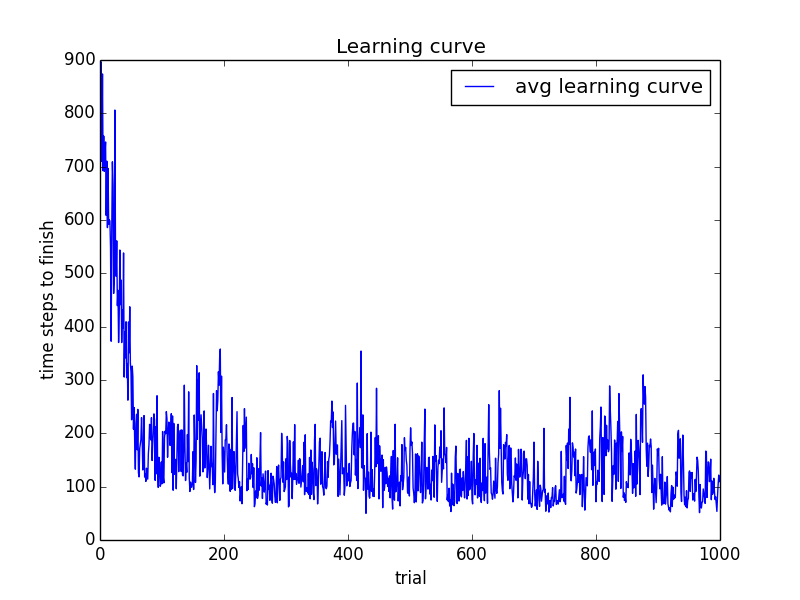
\includegraphics[width=0.8\textwidth]{figures/learning_curve.png}
\caption{\label{fig:lcurve}Learning curve, averaged over $10$ independent
learning agents}
\end{figure}

The learning curve of the implemented algorithm can be seen in the
Figure \ref{fig:lcurve}. It is an average over $10$ independent learning runs in
order to reduce the high oscillations of a single run. The initial drop in the curve
shows how the agent takes less time to 
complete the track. In Fig. \ref{fig:lcurve} the latency decreases from 900 to around 130 time steps on average before the 50th trial. In other words, the agent indeed learns the topology of the track
and the location of the reward. The learning curve plateaus after
approximately $100$ trials and after that the latency stops decreasing and
oscillates instead, between the values of $100$ and $300$. This shows that the agent has learned enough information
about the environment and starts to exploit it extensively. The exploration that
happens ($\epsilon = 0.1$ or 10$\%$ of the time) is not enough to find the better solutions.

\begin{figure}[h!]
\centering
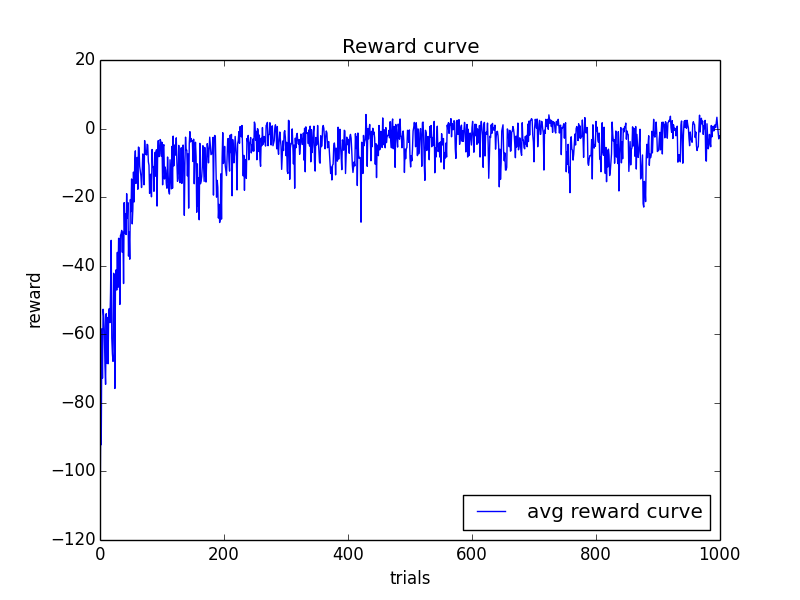
\includegraphics[width=0.8\textwidth]{figures/reward_curve.png}
\caption{\label{fig:rcurve}Reward curve, averaged over 10 independent learning
cars}
\end{figure}

\paragraph{Integrated reward}
The reward curve is plotted in the Figure~\ref{fig:rcurve}. Qualitatively, it resembles
the learning curve, despite being negative and scaled. The consistency between
the two curves confirms the correlation between the reward obtained and the
learning.

\paragraph{Exploration-exploitation}
Exploration-exploitation tradeoff is controlled with $\epsilon$ parameter when
the $\epsilon$-greedy strategy is used. Learning curves for different $\epsilon$
values can be seen in Figure~\ref{fig:eps}. When $\epsilon$ is too small
($\epsilon \sim 0$) algorithm exploits the acquired knowledge at every step. It
often happens that the agent does not explore the majority of solutions and it
is clearly visible from the learning curve in Figure~\ref{fig:eps0} that it did
not gain almost any knowledge about the track. The latency does not decrease and
the variance is large during the learning process. On the other hand, setting
$\epsilon$ to high values ($\epsilon \ge 0.5$) employs too much exploration such
that the agent rarely has the chance to apply what it has learned and wanders
around the map too much, which is also visible from the learning curve
(Figure \ref{fig:eps5} and Figure~\ref{fig:eps10}). The best observed values for
$\epsilon$ are when it is slightly lower than $0.1$, for example $\epsilon =
0.05$ shown in Figure~\ref{fig:eps05}.  One additional insight to the influence
of $\epsilon$ parameter can be observed in Table~\ref{tab:perf}. Same
conclusions could be drawn from that table, the best values again being
$\epsilon \in [0.05, 0.1]$.

In addition, we tried to improve the performance of our agent by decreasing
$\epsilon$ linearly during the learning session, with different starting and
ending values. For some reason, this yields two different behaviors at different
runs. At some times it gives a very good performance, slightly better than
already observed. However, at some other runs it can't seem to learn the good
trajectory and most often (during the learning session) does not even finish the
track. Average performance is always around $135$ and the number of agents
finishing the race is around $90\%$.

\begin{table}[h!]
\centering
\begin{tabular}{|c|c|c|}
\hline
$\epsilon$ & performance & finished \\
\hline
$0.0$ & $549.05$ & $44\%$\\
\hline
$0.05$ & $76.78$ & $100\%$ \\
\hline
$0.1$ & $88.12$ & $100\%$ \\
\hline
$0.2$ & $139.72$ & $94\%$ \\
\hline
$0.5$ & $223.71$ & $91\%$ \\
\hline
$1.0$ & $609.82$ & $35\%$ \\
\hline
\end{tabular}
\caption{\label{tab:perf}Navigation performance with varying
$\epsilon$. For each value of $\epsilon$ we trained $10$ agents. Performance is
measured as the average latency for an agent in the last $10$ trials of any learning
session, provided that the agent finishes the race. The percentage in the third
column shows how many of the observed agents managed to finish the race (and
hence are counted in the average).}
\end{table}

\begin{figure}[h!]
\centering
\begin{subfigure}[b]{0.4\textwidth}
    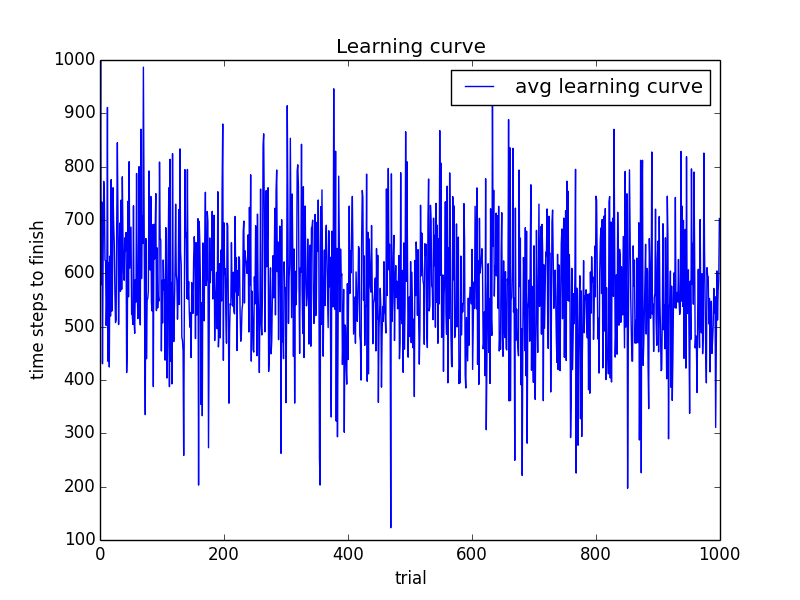
\includegraphics[width=\textwidth]{figures/epsilon_0_learning_curve.png}
    \caption{\label{fig:eps0}$\epsilon = 0$}
\end{subfigure}
~
\begin{subfigure}[b]{0.4\textwidth}
    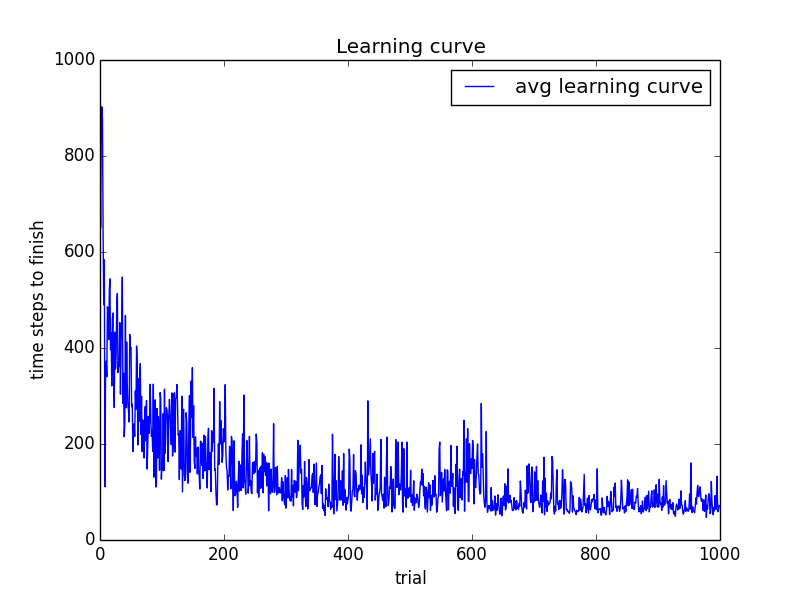
\includegraphics[width=\textwidth]{figures/epsilon_05_learning_curve.png}
    \caption{\label{fig:eps05}$\epsilon = 0.05$}
\end{subfigure}
\begin{subfigure}[b]{0.4\textwidth}
    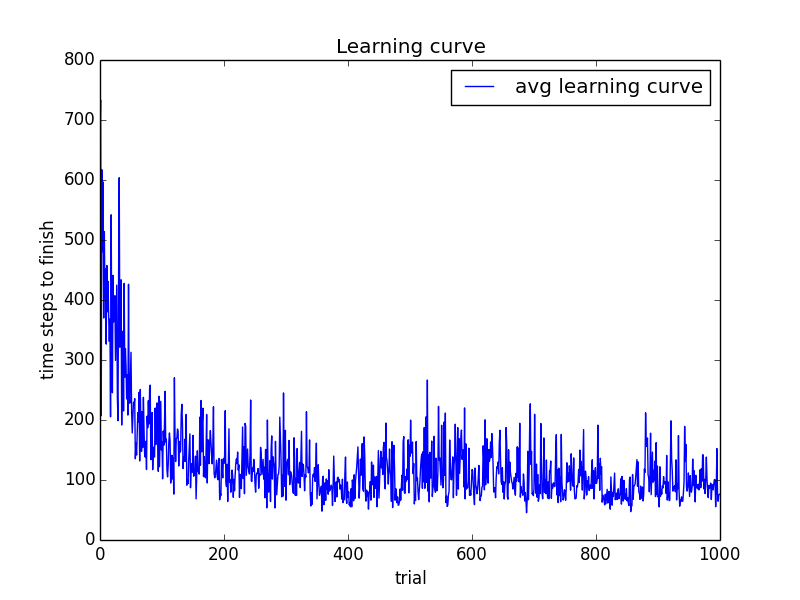
\includegraphics[width=\textwidth]{figures/epsilon_1_learning_curve.png}
    \caption{$\epsilon = 0.1$}
\end{subfigure}
~
\begin{subfigure}[b]{0.4\textwidth}
    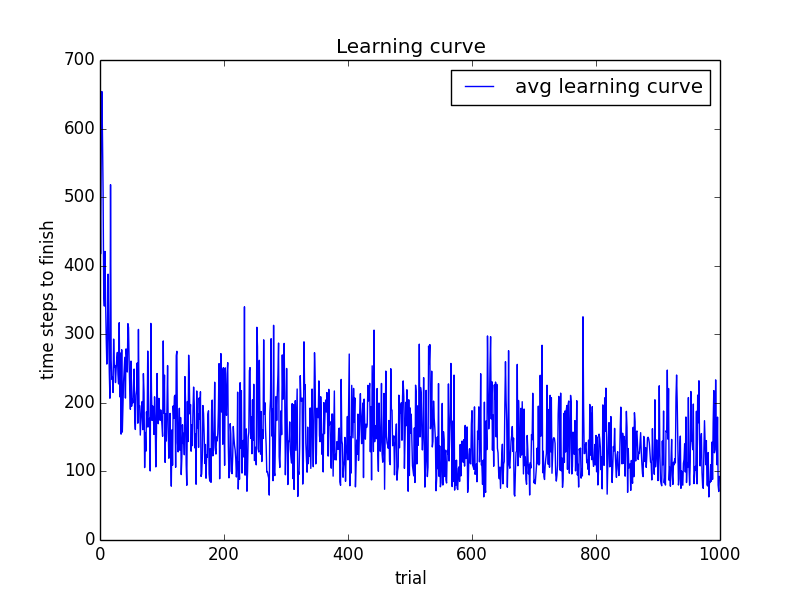
\includegraphics[width=\textwidth]{figures/epsilon_2_learning_curve.png}
    \caption{$\epsilon = 0.2$}
\end{subfigure}
\begin{subfigure}[b]{0.4\textwidth}
    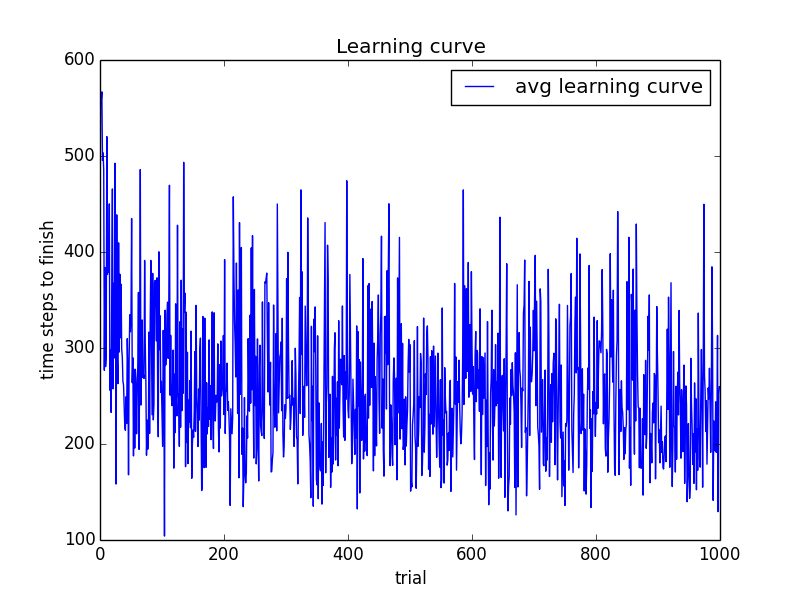
\includegraphics[width=\textwidth]{figures/epsilon_5_learning_curve.png}
    \caption{\label{fig:eps5}$\epsilon = 0.5$}
\end{subfigure}
~
\begin{subfigure}[b]{0.4\textwidth}
    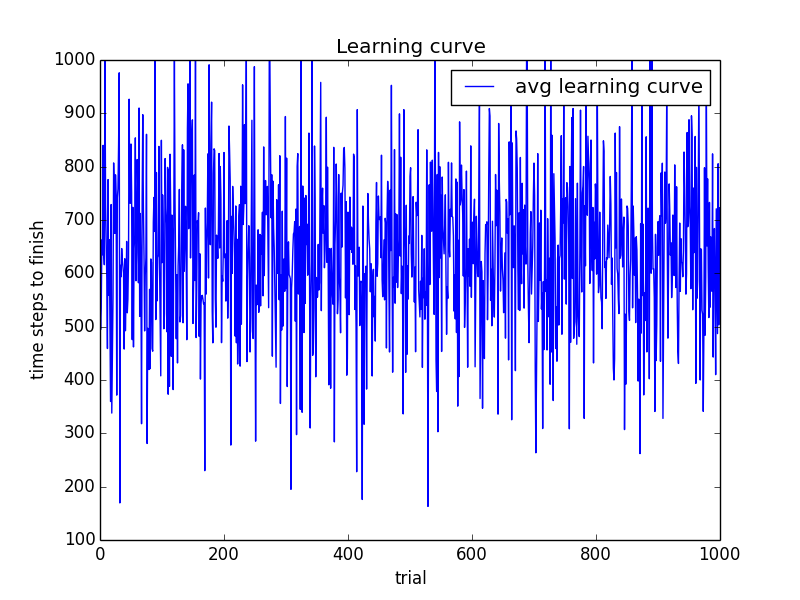
\includegraphics[width=\textwidth]{figures/epsilon_10_learning_curve.png}
    \caption{\label{fig:eps10}$\epsilon = 1.0$}
\end{subfigure}
\caption{\label{fig:eps}Learning curves for different values of $\epsilon$
parameter. This shows the effect of exploration-exploitation tradeoff}
\end{figure}
 


\paragraph{Navigation map}

We show the evolution of the navigation path for the learning agent. At first the agent has no knowledge of the value function describing the track, and we see in Fig. \ref{fig:navmap} that if the agent takes these actions, there are many regions where it could get stuck. With more "experience" (i.e. as learning progresses), agent discovers the reward location and also learns more about the world. We observe that at trial 1000 the value function describing the world provides much more information about the track than it did in the earlier trials, as would be expected after learning. In this last figure, we see the form of a line on the left-hand side where "action" arrows point toward each other. This line outlines actions for a collison-free path.    

A navigation map shows where the agent would go based on the position it is
currently in. Some navigation maps can be seen in the Figure~\ref{fig:navmap}.
It is clearly visible how navigation maps resemble the environment track to
learn in as the learning time passes by.

\begin{figure}[h!]
\centering
\begin{subfigure}[b]{0.6\textwidth}
    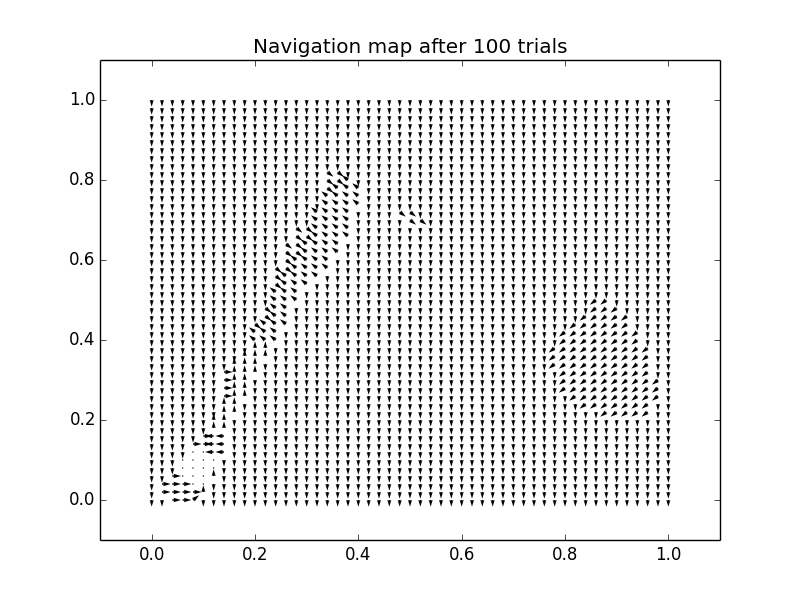
\includegraphics[width=\textwidth]{figures/nmap_100.png}
\end{subfigure}
\begin{subfigure}[b]{0.6\textwidth}
    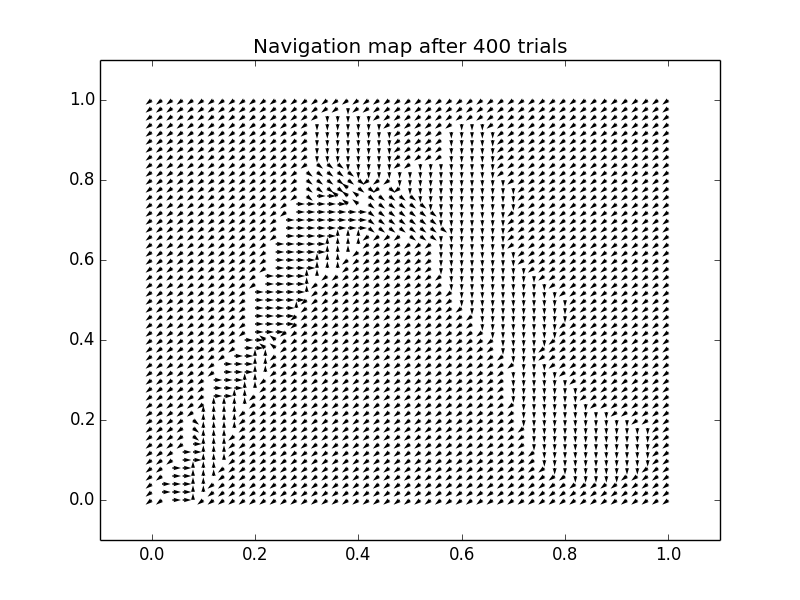
\includegraphics[width=\textwidth]{figures/nmap_400.png}
\end{subfigure}
\begin{subfigure}[b]{0.6\textwidth}
    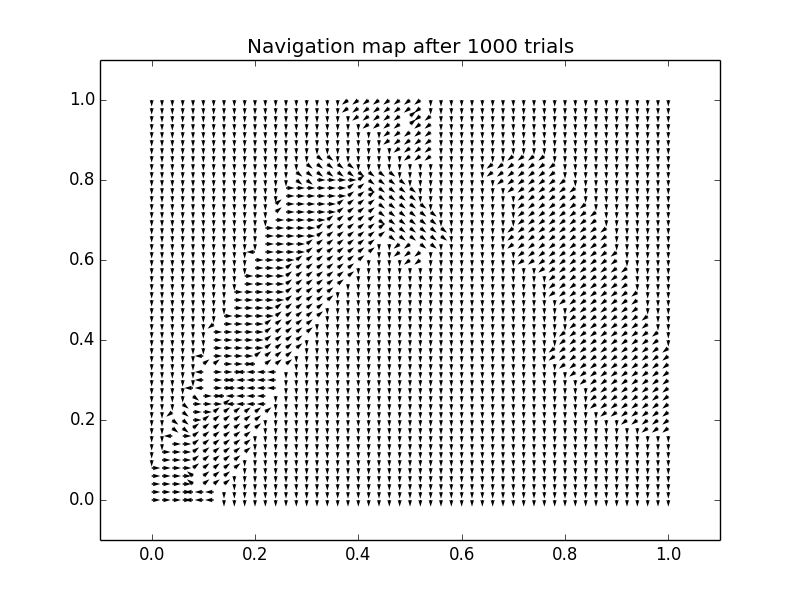
\includegraphics[width=\textwidth]{figures/nmap_1000.png}
\end{subfigure}
\caption{\label{fig:navmap}Navigation maps at different learning stages}
\end{figure}   


%We show the evolution of the learning agent's path over trials. At first the agent has no knowledge of the value function describing the track, so we see it move randomly in Fig. \ref{fig:trial0} until it discovers the reward location in later trials Fig. \ref{fig:trial4}. We observe in Fig. \ref{fig:trial9} it has learned to avoid hitting walls and can reach the reward location using a more efficient path as compared to previous trials. 
%
%\begin{figure}[h!]
%\centering
%\includegraphics[width=0.8\textwidth]{../src/trajectory_0.png}
%\caption{Car trajectory at trial 0. \label{fig:trial0}}
%\end{figure}
%
%
%\begin{figure}[h!]
%\centering
%\includegraphics[width=0.8\textwidth]{../src/trajectory_4.png}
%\caption{Car trajectory at trial 4. \label{fig:trial4}}
%\end{figure}
%
%\begin{figure}[h!]
%\centering
%\includegraphics[width=0.8\textwidth]{../src/trajectory_9.png}
%\caption{Car trajectory at trial 9. \label{fig:trial9}}
%\end{figure}

\section{Car race}
We have modified the car to be rewarded by the amount of time left in the trial rather than an absolute maximum reward value. 
